\documentclass[12pt,a4paper]{article}

% ── Packages ──────────────────────────────────────────────────────────────────
\usepackage[utf8]{inputenc}
\usepackage[T1]{fontenc}
\usepackage[english]{babel}
\usepackage{geometry}
\usepackage{graphicx}
\usepackage{listings}
\usepackage{xcolor}
\usepackage{hyperref}
\usepackage{fancyhdr}
\usepackage{titlesec}
\usepackage{enumitem}
\usepackage{booktabs}
\usepackage{array}
\usepackage{float}
\usepackage{amsmath}
\usepackage{amssymb}
\usepackage{parskip}
\usepackage{mdframed}
\usepackage{tcolorbox}
\usepackage{caption}

\geometry{
    top=2.5cm, bottom=2.5cm,
    left=2.5cm, right=2.5cm,
    headheight=15pt
}

% ── Colors ────────────────────────────────────────────────────────────────────
\definecolor{codebg}{RGB}{245,245,245}
\definecolor{codeframe}{RGB}{200,200,200}
\definecolor{keywordcolor}{RGB}{0,0,180}
\definecolor{commentcolor}{RGB}{0,128,0}
\definecolor{stringcolor}{RGB}{160,32,32}
\definecolor{titleblue}{RGB}{30,60,120}
\definecolor{sectionblue}{RGB}{0,80,160}
\definecolor{warnred}{RGB}{180,0,0}

% ── Listings (C code style) ───────────────────────────────────────────────────
\lstdefinestyle{cstyle}{
    backgroundcolor=\color{codebg},
    frame=single,
    rulecolor=\color{codeframe},
    basicstyle=\ttfamily\small,
    keywordstyle=\color{keywordcolor}\bfseries,
    commentstyle=\color{commentcolor}\itshape,
    stringstyle=\color{stringcolor},
    numberstyle=\tiny\color{gray},
    numbers=left,
    stepnumber=1,
    breaklines=true,
    breakatwhitespace=false,
    tabsize=4,
    showstringspaces=false,
    language=C,
    morekeywords={pid_t, sig_atomic_t, sigaction, siginfo_t, DIR, dirent,
                  ssize_t, off_t, mode_t},
    captionpos=b
}
\lstset{style=cstyle}

% ── Section title formatting ──────────────────────────────────────────────────
\titleformat{\section}
    {\Large\bfseries\color{sectionblue}}
    {\thesection.}{0.5em}{}[\titlerule]

\titleformat{\subsection}
    {\large\bfseries\color{sectionblue!80}}
    {\thesubsection.}{0.5em}{}

\titleformat{\subsubsection}
    {\normalsize\bfseries}
    {\thesubsubsection.}{0.5em}{}

% ── Header / Footer ───────────────────────────────────────────────────────────
\pagestyle{fancy}
\fancyhf{}
\fancyhead[L]{\small CSE344 -- System Programming}
\fancyhead[R]{\small Homework \#2}
\fancyfoot[C]{\thepage}
\renewcommand{\headrulewidth}{0.4pt}

% ── Hyperref setup ────────────────────────────────────────────────────────────
\hypersetup{
    colorlinks=true,
    linkcolor=sectionblue,
    urlcolor=sectionblue,
    pdftitle={CSE344 HW2 Report},
    pdfauthor={Student}
}

% ── tcolorbox styles ──────────────────────────────────────────────────────────
\tcbuselibrary{skins,breakable}
\newtcolorbox{infobox}[1][]{
    colback=blue!5,colframe=sectionblue,
    fonttitle=\bfseries, title=#1,
    breakable
}
\newtcolorbox{warnbox}[1][]{
    colback=red!5,colframe=warnred,
    fonttitle=\bfseries, title=#1,
    breakable
}

% ══════════════════════════════════════════════════════════════════════════════
\begin{document}

% ── Cover Page ────────────────────────────────────────────────────────────────
\begin{titlepage}
    \centering
    \vspace*{1cm}

    {\Huge\bfseries\color{titleblue} Gebze Technical University\\[0.3em]
    Department of Computer Engineering}

    \vspace{1.5cm}
    \rule{\linewidth}{1pt}
    \vspace{0.5cm}

    {\LARGE\bfseries CSE344 -- System Programming}\\[0.5em]
    {\Large Homework \#2}\\[0.3em]
    {\large Signal Handling \& Process Management with \texttt{fork()}}

    \vspace{0.5cm}
    \rule{\linewidth}{1pt}
    \vspace{2cm}

    \begin{tabular}{rl}
        \textbf{Name \& Surname:} & Halit Batuhan ASLAN \\[0.4em]
        \textbf{Student ID:}      & 220104004003 \\[0.4em]
        \textbf{Course:}          & CSE344 -- System Programming \\[0.4em]
        \textbf{Homework:}        & \#2 \\[0.4em]
        \textbf{Due Date:}        & 27 March 2026, 23:59 \\[0.4em]
        \textbf{Instructor:}      & Zehra Bilici \\
    \end{tabular}

    \vfill
    {\large March 2026}
\end{titlepage}

% ── Table of Contents ─────────────────────────────────────────────────────────
\tableofcontents
\newpage

% ══════════════════════════════════════════════════════════════════════════════
\section{Introduction}

This report describes the design and implementation of \texttt{procSearch}, a
multi-process file search tool written in C using Linux system calls.
The program accepts a root directory and a filename pattern, forks a
configurable number of worker processes, and assigns each worker a partition
of the directory tree to search recursively.

\subsection{Program Overview}

\texttt{procSearch} is invoked as follows:

\begin{lstlisting}[language=bash, style=cstyle, caption={Program usage}]
./procSearch -d <root_dir> -n <num_workers> -f <pattern> [-s <min_size_bytes>]
\end{lstlisting}

\begin{description}[leftmargin=2cm]
    \item[\texttt{-d}] Root directory to search (must exist)
    \item[\texttt{-n}] Number of worker processes to fork (2--8 inclusive)
    \item[\texttt{-f}] Filename pattern supporting the \texttt{+} operator
    \item[\texttt{-s}] Optional: match only files with size $\geq$ \textit{min\_size} bytes
\end{description}

\subsection{Overall Design Rationale}

The program is structured into the following modules, each in its own
\texttt{.c}/\texttt{.h} pair:

\begin{center}
\begin{tabular}{ll}
    \toprule
    \textbf{Module} & \textbf{Responsibility} \\
    \midrule
    \texttt{argument\_parsing}    & Command-line parsing via \texttt{getopt()} \\
    \texttt{pattern\_matching}    & Custom \texttt{+} operator regex engine \\
    \texttt{partition\_of\_workers} & Round-robin subdirectory distribution \\
    \texttt{worker}               & \texttt{fork()}, search dispatch, lifecycle \\
    \texttt{searching}            & Recursive directory traversal \\
    \texttt{signals\_handler}     & All four signal handlers \\
    \texttt{print\_result}        & Tree-formatted output \& summary \\
    \bottomrule
\end{tabular}
\end{center}

\newpage

% ══════════════════════════════════════════════════════════════════════════════
\section{Design Decisions}

\subsection{Directory Partitioning}

Before forking, the parent process reads the immediate subdirectories of
\texttt{root\_dir} using \texttt{opendir()} / \texttt{readdir()} and
\texttt{lstat()} to identify directories.
These are distributed among workers in \textbf{round-robin} order.

\begin{infobox}[Key rule confirmed by instructor]
Files located directly inside \texttt{root\_dir} (not in any subdirectory) are
searched by the \textbf{parent process itself} via \texttt{search\_root\_files()}.
Only subdirectories are handed to worker processes.
\end{infobox}

Edge cases handled:
\begin{itemize}
    \item If subdirectory count $<$ \texttt{num\_workers}: worker count is
          reduced and a notice is printed.
    \item If there are no subdirectories at all: the parent searches the root
          directly; no \texttt{fork()} is called.
\end{itemize}

\subsection{Inter-Process Communication via Temporary Files}

Because \texttt{exit()} can only return 8 bits of information
(\texttt{match\_count \% 256}), file paths and scan counts cannot be passed
through the exit status. The design uses temporary files:

\begin{enumerate}
    \item Each worker writes its matches to \texttt{/tmp/worker\_<PID>.txt}.
    \item The first line contains \texttt{Scanned:N} (total files examined).
    \item Subsequent lines contain: \texttt{<PID> <path> (<size> bytes)}.
    \item The parent reads these files after all workers finish, builds the
          tree, then deletes them.
\end{enumerate}

This approach eliminates the need for pipes or shared memory, as confirmed
acceptable by the instructor.

\subsection{Signal Handler Architecture}

All four required signals are implemented using \texttt{sigaction()} (never
\texttt{signal()}) for reliable, portable behaviour.

\begin{warnbox}[Async-signal-safety]
No \texttt{printf()}, \texttt{malloc()}, or other non-async-signal-safe
functions are called inside any signal handler. Handlers only set
\texttt{volatile sig\_atomic\_t} flags or call \texttt{write()} /
\texttt{waitpid()} which are async-signal-safe.
\end{warnbox}

\subsubsection{SIGUSR1 -- Worker Completion}

Workers send \texttt{SIGUSR1} to the parent upon normal completion.
The handler uses \texttt{SA\_SIGINFO} to read the sender's PID
(\texttt{info->si\_pid}), which is stored in the \texttt{expected\_pids[]}
array. A \texttt{workers\_done} counter is incremented atomically.

\subsubsection{SIGCHLD -- Zombie Prevention}

The parent installs a \texttt{SIGCHLD} handler that calls
\texttt{waitpid(-1, \&status, WNOHANG)} in a loop. Inside the handler, if the
terminated PID is found in \texttt{expected\_pids[]} it is a normal finish and
no action is taken. Otherwise an ``unexpected termination'' message is written
to \texttt{stderr} via \texttt{write()}.

\subsubsection{SIGINT -- Graceful Shutdown}

\begin{enumerate}
    \item Parent sends \texttt{SIGTERM} to all workers.
    \item Parent waits 3 seconds (\texttt{sleep(3)}).
    \item Any surviving workers receive \texttt{SIGKILL}.
    \item Parent reads whatever \texttt{worker\_<PID>.txt} files exist
          (workers that had not yet created theirs contribute 0 matches).
    \item A \textbf{partial summary} is printed with the label
          \texttt{--- Summary (partial) ---}.
\end{enumerate}

Workers ignore \texttt{SIGINT} (\texttt{SIG\_IGN}) so that pressing Ctrl+C
does not kill them directly; only the parent decides when to terminate them.

\subsubsection{SIGTERM -- Worker Termination}

The worker sets the \texttt{got\_sigterm} flag. The main search loop checks
this flag at each iteration boundary. Upon detecting the flag, the worker
prints its partial match count, flushes its temporary file, and calls
\texttt{exit(match\_count \% 256)}.

\subsection{Avoiding the \texttt{pause()} Race Condition}

The parent waits for all workers with:

\begin{lstlisting}[caption={Wait loop in worker.c}]
while (workers_done < num_of_workers) {
    if (got_sigint) { ... handle ... return; }
    pause();   /* wakes on any signal */
}
\end{lstlisting}

\texttt{pause()} is used here because \texttt{SIGUSR1} arrives asynchronously
and wakes the call immediately. \texttt{SA\_RESTART} is \textit{not} set for
\texttt{SIGINT} so that \texttt{pause()} returns with \texttt{EINTR} when
Ctrl+C is pressed, allowing the shutdown path to execute without delay.

\subsection{Pattern Matching Engine}

The \texttt{+} operator is implemented from scratch in
\texttt{pattern\_matching.c} without any regex library.

\begin{infobox}[Instructor clarification]
The \texttt{+} operator applies to the \textbf{single character immediately to
its left}. Example: \texttt{rep+ort} matches \texttt{report},
\texttt{repport}, \texttt{reppport} (one or more \textbf{p}), \textbf{not}
\texttt{repoort} or \texttt{repoooort}.
\end{infobox}

The algorithm uses recursive backtracking:
\begin{enumerate}
    \item For each starting position in the filename, attempt to match the
          full pattern via \texttt{match\_at\_recursive()}.
    \item When a \texttt{+} is encountered, greedily consume as many copies of
          the preceding character as possible, then backtrack from maximum to
          minimum (1) to find a valid continuation.
    \item Comparison is case-insensitive via \texttt{tolower()}.
\end{enumerate}

\newpage

% ══════════════════════════════════════════════════════════════════════════════
\section{Mandatory Test Scenario \& Screenshots}

All tests were conducted on Debian 11 (64-bit) in VirtualBox using the
mandatory directory structure specified in the assignment.

% ── Screenshot 1 ──────────────────────────────────────────────────────────────
\subsection{Screenshot 1 -- Test Directory Setup and Compilation}

The test directory tree under \texttt{/tmp/crawltest} was created with the
following commands, followed by a successful \texttt{make} with zero warnings:

\begin{lstlisting}[language=bash, caption={Setup and build commands}]
mkdir -p /tmp/crawltest/alpha/sub1
mkdir -p /tmp/crawltest/beta
mkdir -p /tmp/crawltest/gamma
mkdir -p /tmp/crawltest/delta

echo 'quarterly report data' > /tmp/crawltest/alpha/report.txt
touch /tmp/crawltest/alpha/notes.md
echo 'old duplicate report'  > /tmp/crawltest/alpha/sub1/repoort.txt
touch /tmp/crawltest/alpha/sub1/image.png
touch /tmp/crawltest/beta/error_log.txt
echo 'final version'         > /tmp/crawltest/beta/report_final.txt
echo 'archived report'       > /tmp/crawltest/gamma/repoooort.txt
touch /tmp/crawltest/gamma/data.csv
touch /tmp/crawltest/delta/summary.txt

find /tmp/crawltest | sort   # verify tree
make clean && make            # compile with -Wall, 0 warnings
\end{lstlisting}

\begin{figure}[H]
    \centering
    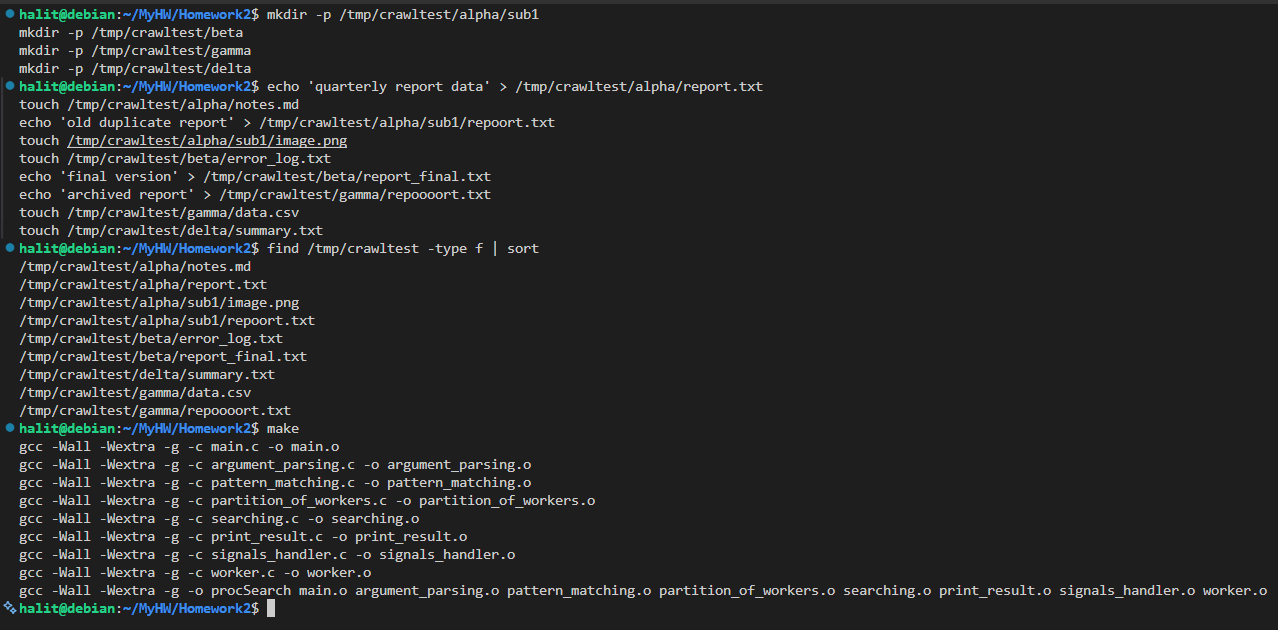
\includegraphics[width=\linewidth]{testFileCreation.png}
    \caption{Screenshot 1 -- Directory tree verified with \texttt{find} and
             project compiled with zero \texttt{-Wall} warnings}
\end{figure}

% ── Screenshot 2 ──────────────────────────────────────────────────────────────
\subsection{Screenshot 2 -- Pattern Search and Size Filter Tests}

Two searches are run back to back.

\textbf{Test A} -- Basic pattern \texttt{rep+ort} (no size filter):

\begin{lstlisting}[language=bash, caption={Test A: basic pattern search}]
./procSearch -d /tmp/crawltest -n 3 -f 'rep+ort'
\end{lstlisting}

Per the instructor's clarification, \texttt{+} applies to the character
immediately to its left (\texttt{p}), so only filenames containing one or more
consecutive \texttt{p} after \texttt{re} are matched:

\begin{itemize}
    \item \texttt{alpha/report.txt} \checkmark\ -- contains \texttt{rep\underline{p}ort} (single \texttt{p})
    \item \texttt{beta/report\_final.txt} \checkmark\ -- same pattern
    \item \texttt{alpha/sub1/repoort.txt} \texttimes\ -- repeated \texttt{o}, not \texttt{p}
    \item \texttt{gamma/repoooort.txt} \texttimes\ -- repeated \texttt{o}, not \texttt{p}
\end{itemize}

\textbf{Test B} -- Same pattern with \texttt{-s 15} size filter:

\begin{lstlisting}[language=bash, caption={Test B: size filter -s 15}]
./procSearch -d /tmp/crawltest -n 3 -f 'rep+ort' -s 15
\end{lstlisting}

\begin{itemize}
    \item \texttt{report.txt}: content \texttt{'quarterly report data'} = 22 bytes \checkmark
    \item \texttt{report\_final.txt}: content \texttt{'final version'} = 14 bytes \texttimes\ (below threshold)
\end{itemize}

\begin{figure}[H]
    \centering
    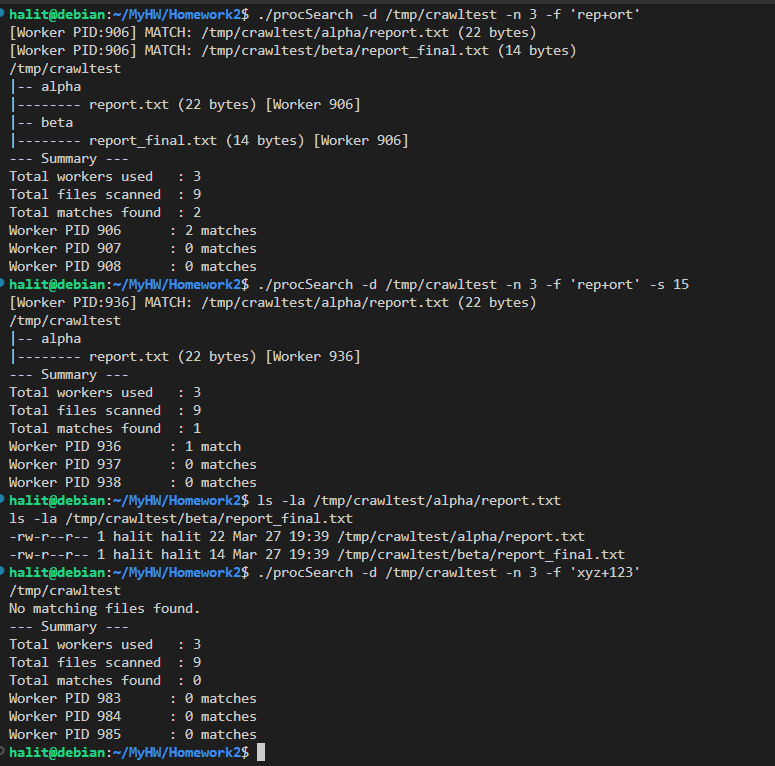
\includegraphics[width=\linewidth]{firstTests.png}
    \caption{Screenshot 2 -- Test A (\texttt{rep+ort}) and Test B (\texttt{-s~15})
             showing correct tree output and summary for each run}
\end{figure}

% ── Screenshot 3 ──────────────────────────────────────────────────────────────
\subsection{Screenshot 3 -- SIGINT Graceful Shutdown}

The program is run against a large directory so it stays alive long enough to
receive Ctrl+C:

\begin{lstlisting}[language=bash, caption={SIGINT test on large directory}]
./procSearch -d /usr/share/doc -n 4 -f 'read+me'
# Press Ctrl+C while workers are still running
\end{lstlisting}

Expected behaviour:
\begin{enumerate}
    \item Parent prints \texttt{[Parent] SIGINT received. Terminating all workers...}
    \item Parent sends \texttt{SIGTERM} to each worker; workers print their
          partial match count and exit.
    \item After 3 seconds any survivors receive \texttt{SIGKILL}.
    \item Parent collects available \texttt{worker\_<PID>.txt} files and prints
          \texttt{--- Summary (partial) ---}.
\end{enumerate}

\begin{figure}[H]
    \centering
    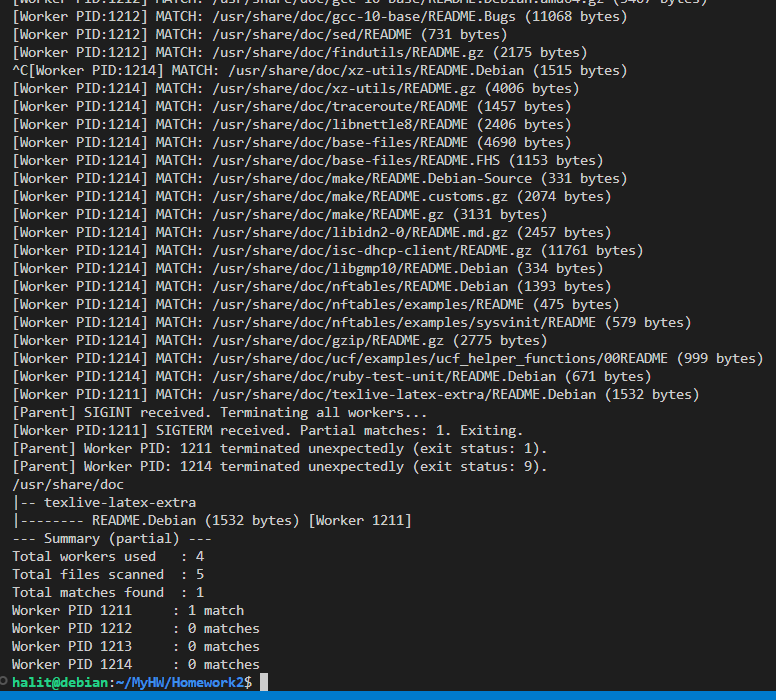
\includegraphics[width=\linewidth]{sigintControlOutput.png}
    \caption{Screenshot 3 -- Ctrl+C received; workers terminated cleanly;
             partial summary printed to stdout}
\end{figure}

% ── Screenshot 4 ──────────────────────────────────────────────────────────────
\subsection{Screenshot 4 -- No Zombie Processes}

Immediately after the SIGINT test, the process table is inspected to confirm
that no zombie (\texttt{Z}) processes remain:

\begin{lstlisting}[language=bash, caption={Zombie verification commands}]
ps -ef | grep procSearch
ps -ef | grep Z | grep -v grep
\end{lstlisting}

A clean result (no output from the second command) confirms that the
\texttt{SIGCHLD} handler successfully called \texttt{waitpid(WNOHANG)} for
every terminated child, preventing zombie accumulation.

\begin{figure}[H]
    \centering
    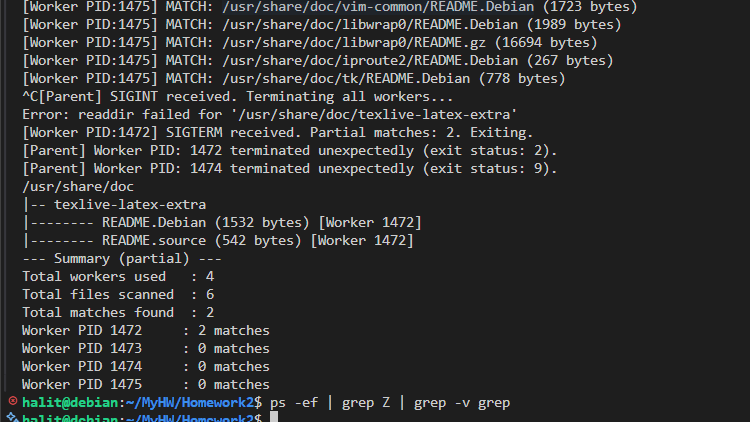
\includegraphics[width=\linewidth]{sigintControlOutputNoZombie.png}
    \caption{Screenshot 4 -- \texttt{ps} output confirms zero zombie processes
             after shutdown}
\end{figure}

\newpage

% ══════════════════════════════════════════════════════════════════════════════
\section{Conclusion}

\subsection{Challenges Faced and How They Were Resolved}

\subsubsection{Pattern Matching: Multiple \texttt{+} Operators and Backtracking}

The \texttt{+} operator was first introduced in Homework \#1 (\texttt{myFind}),
where it was implemented as a simple greedy substring search. That initial
implementation worked correctly for single-\texttt{+} patterns such as
\texttt{lo+g}, but proved insufficient once patterns with multiple \texttt{+}
operators were considered in this homework.

The critical failure case was a pattern like \texttt{rep+p}, which should match
\texttt{reppp}, \texttt{repppp}, and so on. The greedy approach consumed all
consecutive \texttt{p} characters for the first \texttt{+}, leaving none for
the literal \texttt{p} that followed, causing the match to fail incorrectly.
For example:

\begin{center}
\begin{tabular}{lll}
    \toprule
    \textbf{Pattern} & \textbf{Input} & \textbf{Greedy (wrong)} \\
    \midrule
    \texttt{rep+p} & \texttt{reppp} & Fails --- all \texttt{p}s consumed by \texttt{+} \\
    \texttt{er+ro+r} & \texttt{errroor} & Fails --- \texttt{r}s consumed, none left for \texttt{ro} \\
    \bottomrule
\end{tabular}
\end{center}

The solution was to replace the greedy strategy with \textbf{recursive
backtracking} inside \texttt{match\_at\_recursive()}. When a \texttt{+} is
encountered, the engine first counts the maximum number of consecutive
matching characters (\texttt{max\_k}), then tries each count from
\texttt{max\_k} down to \texttt{1}, recursing into the remainder of the
pattern at each attempt. This guarantees that a valid split is always found
if one exists:

\begin{lstlisting}[caption={Backtracking loop in pattern\_matching.c}]
int max_k = 0;
while (t + max_k < text_len && is_same(text[t + max_k], repeat_char))
    max_k++;

/* Try from maximum down to 1 -- prevents greedy over-consumption */
for (int k = max_k; k >= 1; k--) {
    int res = match_at_recursive(text, text_len, t + k,
                                 pattern, pat_len, p + 2);
    if (res != -1) return res;
}
return -1;
\end{lstlisting}

Additionally, the assignment PDF contained a misleading example: \texttt{rep+ort}
was shown matching \texttt{repoort}, implying that \texttt{+} applied to
\texttt{o}. The instructor later clarified that \texttt{+} always applies to
the \textbf{single character immediately to its left}, so \texttt{rep+ort}
correctly matches \texttt{report}, \texttt{repport}, \texttt{reppport} (one
or more \texttt{p}), not \texttt{repoort}. The implementation reflects this
corrected specification. This experience was directly informed by the pattern
matching work carried out in Homework \#1, where the same \texttt{+} semantics
were first established.

\subsubsection{Async-Signal-Safety}

Ensuring that no signal handler violated POSIX async-signal-safety rules was
one of the most demanding constraints. In Homework \#1, signal handling was
limited to \texttt{SIGINT} for clean-up on Ctrl+C, and the handler was
relatively straightforward. Homework \#2 requires four distinct signals
(\texttt{SIGUSR1}, \texttt{SIGINT}, \texttt{SIGTERM}, \texttt{SIGCHLD}),
each with its own logic, which made the safety requirements considerably harder
to satisfy.

The key violations to avoid were:
\begin{itemize}
    \item Calling \texttt{printf()} or \texttt{fprintf()} inside any handler
          (not async-signal-safe).
    \item Calling \texttt{snprintf()} to format PID numbers for error messages
          (also not safe).
    \item Allocating or freeing heap memory inside a handler.
\end{itemize}

All of these were resolved by the following strategy:
\begin{enumerate}
    \item Handlers only set \texttt{volatile sig\_atomic\_t} flags
          (\texttt{got\_sigint}, \texttt{got\_sigterm}, \texttt{workers\_done})
          or call explicitly safe functions (\texttt{write()},
          \texttt{waitpid()}, \texttt{kill()}).
    \item A custom \texttt{int\_to\_str()} function was written to convert
          integer PIDs into character buffers without using any stdio function,
          allowing the \texttt{SIGCHLD} handler to write formatted messages to
          \texttt{stderr} via \texttt{write()} safely.
    \item All formatted output (match lines, summary, tree) is produced in the
          main execution path, never inside a handler.
\end{enumerate}

\subsubsection{SIGINT: Graceful Shutdown and Partial Summary}

Handling \texttt{SIGINT} correctly required coordinating three separate
concerns that do not arise in simpler programs:

\textbf{(1) Propagation to workers.}
Workers ignore \texttt{SIGINT} (\texttt{SIG\_IGN}) so that Ctrl+C in the
terminal does not kill them directly. Only the parent receives \texttt{SIGINT}
and decides to forward \texttt{SIGTERM} (with a 3-second grace period) and
then \texttt{SIGKILL} to any survivors. This prevents workers from being
terminated before they can flush their partial results to disk.

\textbf{(2) Partial file collection.}
After the grace period, some workers may not have created their
\texttt{worker\_<PID>.txt} file yet (e.g., if they were still in the middle of
opening a directory). Per instructor clarification, such workers contribute
0 to the match and scan counts. The parent simply skips missing files during
the collection phase.

\textbf{(3) Interrupting \texttt{pause()}.}
The parent waits for worker completion using \texttt{pause()}, which blocks
until any signal arrives. For \texttt{SIGUSR1} this is the intended behaviour.
For \texttt{SIGINT}, however, it is essential that \texttt{pause()} returns
immediately so the shutdown sequence can begin. This is achieved by installing
the \texttt{SIGINT} handler \textit{without} \texttt{SA\_RESTART}: when
\texttt{SIGINT} arrives, \texttt{pause()} returns with \texttt{EINTR}, the
main loop detects \texttt{got\_sigint == 1}, and shutdown proceeds without
any delay.

\subsubsection{SIGCHLD vs.\ SIGUSR1 Disambiguation}

A subtlety that was not present in Homework \#1 (which had no child processes)
is that a worker finishing normally triggers \textit{two} signals at the parent:
\texttt{SIGUSR1} (explicitly sent by the worker) and \texttt{SIGCHLD}
(automatically sent by the kernel when any child exits). Without bookkeeping,
the \texttt{SIGCHLD} handler would incorrectly classify every normal exit as
an unexpected termination and log a spurious error to \texttt{stderr}.

The solution uses an \texttt{expected\_pids[]} array. The \texttt{SIGUSR1}
handler (which uses \texttt{SA\_SIGINFO} to read the sender's PID from
\texttt{info->si\_pid}) records each finishing worker's PID in this array.
The \texttt{SIGCHLD} handler then checks: if the PID returned by
\texttt{waitpid()} is in \texttt{expected\_pids[]}, the exit was normal and
no message is logged; otherwise, an unexpected termination message is written
to \texttt{stderr}.

\subsubsection{Reuse of Components from Homework \#1}

Several components of \texttt{procSearch} evolved directly from the
\texttt{myFind} implementation in Homework \#1:

\begin{itemize}
    \item \textbf{Recursive directory traversal.}
          The \texttt{opendir()} / \texttt{readdir()} / \texttt{lstat()} loop
          pattern, including the \texttt{errno} check after \texttt{readdir()}
          returns \texttt{NULL} and the skipping of \texttt{.} and \texttt{..},
          was taken directly from the Homework \#1 traversal code and reused
          in \texttt{searching.c}.

    \item \textbf{Tree-formatted output.}
          Homework \#1 required a tree display with increasing dash indentation
          per depth level. The same indentation logic (6 dashes per additional
          level) was carried over into \texttt{print\_result.c},
          extended to also display the responsible worker PID and file size
          alongside each match.

    \item \textbf{Pattern matching foundation.}
          The case-insensitive character comparison (\texttt{tolower()}) and
          the substring-search outer loop (trying every starting position in
          the filename) were established in Homework \#1. Homework \#2 extended
          this foundation with recursive backtracking to handle multiple
          \texttt{+} operators correctly.

    \item \textbf{Argument parsing.}
          The \texttt{getopt()} skeleton and the validation logic
          (required arguments, range checks, trailing slash removal) were
          adapted from the Homework \#1 argument parser.
\end{itemize}

\subsection{Summary}

The implementation satisfies all graded components: pattern matching with the
\texttt{+} operator (with backtracking for multiple operators), round-robin
directory partitioning, worker processes with \texttt{fork()}, all four signal
handlers (\texttt{SIGUSR1}, \texttt{SIGINT}, \texttt{SIGTERM},
\texttt{SIGCHLD}) implemented with full async-signal-safety, tree-formatted
output with worker attribution, and both full and partial summaries. Building
on the foundation established in Homework \#1 allowed the more complex
multi-process and signal-handling aspects of this assignment to be developed
with greater confidence and reduced risk of error.

\end{document}